\documentclass[conference]{IEEEtran}

\usepackage{cite}
\usepackage{url}
\usepackage[cmex10]{amsmath}
\usepackage{amssymb}
\usepackage{multirow}
\interdisplaylinepenalty=2500

% *** GRAPHICS RELATED PACKAGES ***
%
\ifCLASSINFOpdf
  \usepackage[pdftex]{graphicx}
  % declare the path(s) where your graphic files are
  % \graphicspath{{../pdf/}{../jpeg/}}
  % and their extensions so you won't have to specify these with
  % every instance of \includegraphics
  % \DeclareGraphicsExtensions{.pdf,.jpeg,.png}
\else
  % or other class option (dvipsone, dvipdf, if not using dvips). graphicx
  % will default to the driver specified in the system graphics.cfg if no
  % driver is specified.
  % \usepackage[dvips]{graphicx}
  % declare the path(s) where your graphic files are
  % \graphicspath{{../eps/}}
  % and their extensions so you won't have to specify these with
  % every instance of \includegraphics
  % \DeclareGraphicsExtensions{.eps}
\fi



% *** SPECIALIZED LIST PACKAGES ***
%
%\usepackage{algpseudocode}
% algorithmic.sty was written by Peter Williams and Rogerio Brito.
% This package provides an algorithmic environment fo describing algorithms.
% You can use the algorithmic environment in-text or within a figure
% environment to provide for a floating algorithm. Do NOT use the algorithm
% floating environment provided by algorithm.sty (by the same authors) or
% algorithm2e.sty (by Christophe Fiorio) as IEEE does not use dedicated
% algorithm float types and packages that provide these will not provide
% correct IEEE style captions. The latest version and documentation of
% algorithmic.sty can be obtained at:
% http://www.ctan.org/tex-archive/macros/latex/contrib/algorithms/
% There is also a support site at:
% http://algorithms.berlios.de/index.html
% Also of interest may be the (relatively newer and more customizable)
% algorithmicx.sty package by Szasz Janos:
% http://www.ctan.org/tex-archive/macros/latex/contrib/algorithmicx/




% *** ALIGNMENT PACKAGES ***
%
%\usepackage{array}
% Frank Mittelbach's and David Carlisle's array.sty patches and improves
% the standard LaTeX2e array and tabular environments to provide better
% appearance and additional user controls. As the default LaTeX2e table
% generation code is lacking to the point of almost being broken with
% respect to the quality of the end results, all users are strongly
% advised to use an enhanced (at the very least that provided by array.sty)
% set of table tools. array.sty is already installed on most systems. The
% latest version and documentation can be obtained at:
% http://www.ctan.org/tex-archive/macros/latex/required/tools/


%\usepackage{mdwmath}
%\usepackage{mdwtab}
% Also highly recommended is Mark Wooding's extremely powerful MDW tools,
% especially mdwmath.sty and mdwtab.sty which are used to format equations
% and tables, respectively. The MDWtools set is already installed on most
% LaTeX systems. The lastest version and documentation is available at:
% http://www.ctan.org/tex-archive/macros/latex/contrib/mdwtools/


% IEEEtran contains the IEEEeqnarray family of commands that can be used to
% generate multiline equations as well as matrices, tables, etc., of high
% quality.


%\usepackage{eqparbox}
% Also of notable interest is Scott Pakin's eqparbox package for creating
% (automatically sized) equal width boxes - aka "natural width parboxes".
% Available at:
% http://www.ctan.org/tex-archive/macros/latex/contrib/eqparbox/





% *** SUBFIGURE PACKAGES ***
%\usepackage[tight,footnotesize]{subfigure}
% subfigure.sty was written by Steven Douglas Cochran. This package makes it
% easy to put subfigures in your figures. e.g., "Figure 1a and 1b". For IEEE
% work, it is a good idea to load it with the tight package option to reduce
% the amount of white space around the subfigures. subfigure.sty is already
% installed on most LaTeX systems. The latest version and documentation can
% be obtained at:
% http://www.ctan.org/tex-archive/obsolete/macros/latex/contrib/subfigure/
% subfigure.sty has been superceeded by subfig.sty.



% subfig.sty, also written by Steven Douglas Cochran, is the modern
% replacement for subfigure.sty. However, subfig.sty requires and
% automatically loads Axel Sommerfeldt's caption.sty which will override
% IEEEtran.cls handling of captions and this will result in nonIEEE style
% figure/table captions. To prevent this problem, be sure and preload
% caption.sty with its "caption=false" package option. This is will preserve
% IEEEtran.cls handing of captions. Version 1.3 (2005/06/28) and later 
% (recommended due to many improvements over 1.2) of subfig.sty supports
% the caption=false option directly:
\usepackage[caption=false,font=footnotesize]{subfig}
%
% The latest version and documentation can be obtained at:
% http://www.ctan.org/tex-archive/macros/latex/contrib/subfig/
% The latest version and documentation of caption.sty can be obtained at:
% http://www.ctan.org/tex-archive/macros/latex/contrib/caption/




% *** FLOAT PACKAGES ***
%
%\usepackage{fixltx2e}
% fixltx2e, the successor to the earlier fix2col.sty, was written by
% Frank Mittelbach and David Carlisle. This package corrects a few problems
% in the LaTeX2e kernel, the most notable of which is that in current
% LaTeX2e releases, the ordering of single and double column floats is not
% guaranteed to be preserved. Thus, an unpatched LaTeX2e can allow a
% single column figure to be placed prior to an earlier double column
% figure. The latest version and documentation can be found at:
% http://www.ctan.org/tex-archive/macros/latex/base/



%\usepackage{stfloats}
% stfloats.sty was written by Sigitas Tolusis. This package gives LaTeX2e
% the ability to do double column floats at the bottom of the page as well
% as the top. (e.g., "\begin{figure*}[!b]" is not normally possible in
% LaTeX2e). It also provides a command:
%\fnbelowfloat
% to enable the placement of footnotes below bottom floats (the standard
% LaTeX2e kernel puts them above bottom floats). This is an invasive package
% which rewrites many portions of the LaTeX2e float routines. It may not work
% with other packages that modify the LaTeX2e float routines. The latest
% version and documentation can be obtained at:
% http://www.ctan.org/tex-archive/macros/latex/contrib/sttools/
% Documentation is contained in the stfloats.sty comments as well as in the
% presfull.pdf file. Do not use the stfloats baselinefloat ability as IEEE
% does not allow \baselineskip to stretch. Authors submitting work to the
% IEEE should note that IEEE rarely uses double column equations and
% that authors should try to avoid such use. Do not be tempted to use the
% cuted.sty or midfloat.sty packages (also by Sigitas Tolusis) as IEEE does
% not format its papers in such ways.

\hyphenation{op-tical net-works semi-conduc-tor}


\begin{document}
%
% can use linebreaks \\ within to get better formatting as desired
\title{Improving Sensor Data Delivery During Disaster Scenarios with Resilient Overlay Networks}
%\title{Improving Many-to-one Communication During Disaster Scenarios with Resilient Overlay Networks}

\author{\IEEEauthorblockN{Kyle E. Benson and Nalini Venkatasubramanian}
\IEEEauthorblockA{Donald Bren School of Information and Computer Sciences\\
University of California, Irvine\\
%Irvine, California 92697--3425\\
Email: kebenson@ics.uci.edu, nalini@ics.uci.edu}}

% use for special paper notices
%\IEEEspecialpapernotice{(Invited Paper)}


\maketitle


%%%%%%%%%%%%%%%%%%%%%%%%%%%%%%%%%%%%%%%%%%%%%%%%%%%%%%%
%%%%%%%%%      MACROS
%%%%%%%%%%%%%%%%%%%%%%%%%%%%%%%%%%%%%%%%%%%%%%%%%%%%%%%
\newcommand{\numruns}{200 }
\newcommand{\pfail}{p(fail) }

%%%%%%%%%%%%%%%%%%%%%%%%%%%%%%%%%%%%%%%%%%%%%%%%%%%%%%%


\begin{abstract}
%\boldmath

In this paper, we consider many-to-one communication, in particular Internet-connected sensors and their relation to disaster response.
We explore the application of resilient overlay networks to aid these devices, or individuals if we consider participatory sensing,  in quickly and effectively routing around geographically correlated failures in the underlying network infrastructure, as would occur during a large-scale natural disaster.
We develop a formal model of this system, a heuristic for choosing overlay paths without relying on any knowledge of the underlying network infrastructure, and show its merit through simulations using real Internet topologies.

\end{abstract}

% For peer review papers, you can put extra information on the cover
% page as needed:
% \ifCLASSOPTIONpeerreview
% \begin{center} \bfseries EDICS Category: 3-BBND \end{center}
% \fi
%
% For peerreview papers, this IEEEtran command inserts a page break and
% creates the second title. It will be ignored for other modes.
\IEEEpeerreviewmaketitle



\section{Introduction}
% no \IEEEPARstart

With the increasing availability and decreasing cost of microelectromechanical systems (MEMS) sensors, several projects have begun exploring the use of these devices in Internet-connected distributed sensing efforts.
The Quake-Catcher Network \cite{qcn} and Community Seismic Network \cite{csn_site} utilize small inexpensive accelerometers attached to volunteers' computers to monitor seismic activity.
When they detect abnormal ground motion, indicative of a possible seismic event, these hosts report to a central server that processes the information and determines if an earthquake has occurred.
Other such devices, whose information could help understand regional impact of phenomena, include weather stations, pollution detectors, and geiger counters \cite{caltech_sensors}.

We believe that the domain of disaster response could benefit from the inputs of these community scale networked sensors.
Such sensor networks could potentially detect these events' onset and warn possibly affected individuals to find shelter, as well as aid first responders through increased situational awareness.
However, network failures can severely hamper these networks' ability to gather useful information in a timely manner, especially important for those aimed at monitoring fast-moving destructive physical phenomena such as earthquakes and floods.
Such events often result in large-scale geographically correlated failures in addition to serious network congestion as individuals contact each other or request help, exacerbating failures or tying up channels entirely.

Many previous projects have explored resilience to failures in the Internet, although few have addressed large-scale geographically correlated failures.
Most of these works aim to formally model failures and identify strategies for designing more reliable network infrastructure.
For example, \cite{geocorrelated} studied regional failures by defining line segments that cut any intersecting links in the graph representative of the network topology under consideration.
Some of the most devastatingly impacting link cuts possible in a particular network provider were identified and categorized in \cite{net_disaster_planning} to aid in planning more resilient networks.
Both \cite{model_analysis} and \cite{resilience_survey} discuss general challenges to networked systems and discuss the proposed \emph{ResiliNets} framework, which aims to formalize the steps and strategies involved in designing and maintaining more robust networks.

\begin{figure}[!t]
\centering
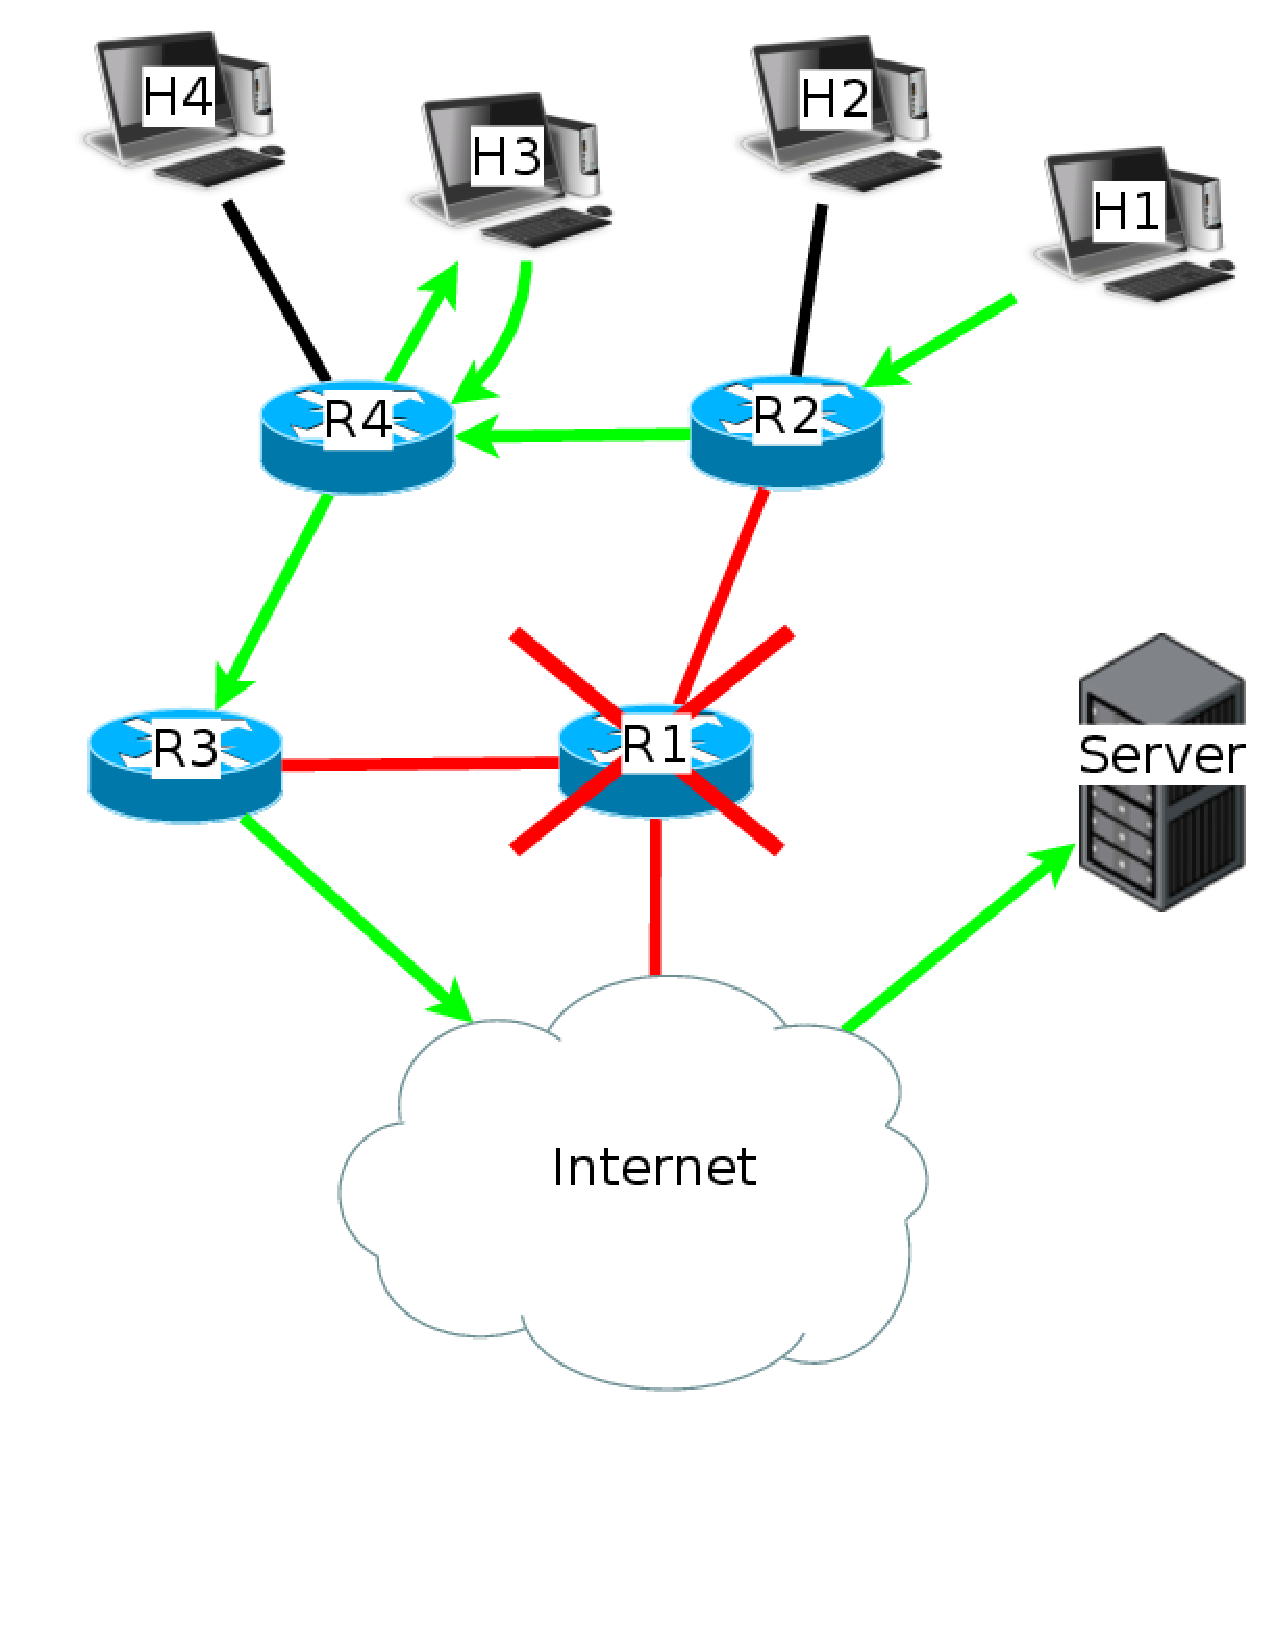
\includegraphics[width=2.5in]{overlay_path.pdf}
\caption{An overlay routing example.  Consider R1, R2, R3, and R4 are routers.  R1 (crossed out) has failed and host H1's normal (shortest) path to the server is unavailable.  Instead, it can route through nearby nodes in the order shown (R2, R4, H3, R4, R3, through the Internet and finally to the server).  H3 serves as an intermediary hop so that H1 can target a different path along the underlying network, without the network knowing about it.}
\label{fig_overlay_path}
\end{figure}

%%%%%%%%%%
\subsection{Resilient Overlay Networks}

In this paper, we explore the creation and use of resilient overlay networks (RONs) to address large-scale disasters and the resultant failures that hamper sensor devices', as well as responders', ability to deliver data over the Internet backbone.
Previous research \cite{ron,reactive_routing} has shown that these overlay networks can help route packets along alternative communication paths when the primary one is damaged, unavailable, or simply congested.
This particularly helps while routing protocols still have not converged and established new end-to-end paths.

%TODO: find the 40 seconds to SON speaker on 11/1 was referring to

When a particular link becomes unavailable, whether due to a physical failure or congestion, the network's underlying routing protocols may take several minutes to find an alternative route.
Several case studies have identified serious problems with routing over the Internet, such as \cite{routing_resilience_analysis} that discovered several paths hopping to other continents unnecessarily after a major earthquake in Taiwan.
This paper also determined that BGP policies significantly reduced Internet resilience due to disallowing certain paths.
Most visible failures were found to not exceed 5-15 minutes in \cite{reactive_routing} and BGP route update convergence was found to take up to 15 minutes after a fault in \cite{route_convergence}.
During this time, some end-to-end connections may be unavailable because certain paths are non-functional but others may exist that the routing infrastructure is not yet aware of.

%TODO: 6 hours of downtime from that speaker

In RONs, routers try to find an alternative path when the main one fails to deliver a packet, as shown in Figure \ref{fig_overlay_path}.
They attempt to make contact with another node in the overlay to see if that node is reachable and has a working path to the desired destination.
If it does, then the traffic is routed through this intermediate node to the destination until a more direct path becomes available or less congested.
Adding this level of intelligence to the routing infrastructure may incur large amounts of additional complexity and cost, but it can also be accomplished with simple end hosts in a peer-to-peer-like fashion.
Deploying end hosts for the specific purpose of establishing a RON, or using those that are already part of a distributed sensing effort for this purpose as well, could possibly increase the reliability of a system without having to modify any of the routers in the underlying physical network.


%%%%%%%%%%%%%%%%%%%%%%%%%%%%%%%%%%%%%%%%%%%%%%%%%%%%%%%%%%%%%%%%%%%%%%%%%%%%%%%%%%%%%%%%%%%%%%%%%%%%%%%%%%%%%%%%%%%%

% 
% \section{Related Work}
% \label{related work}
% 
% Many previous projects have explored resilience to failures in the Internet, although few have addressed large-scale geographically correlated failures.
% Most of these works aim to formally model failures and identify strategies for designing more reliable network infrastructure.
% For example, \cite{geocorrelated} studied regional failures by defining line segments that cut any intersecting links in the graph representative of the network topology under consideration.
% The most devastatingly impacting link cuts possible in a particular network provider were identified and categorized in \cite{net_disaster_planning} to aid in planning more resilient networks.
% Both \cite{model_analysis} and \cite{resilience_survey} discuss general challenges to networked systems and discuss the proposed \emph{ResiliNets} framework, which aims to formalize the steps and strategies involved in designing and maintaining more robust networks.

% Several case studies have identified serious problems with routing over the Internet, such as \cite{routing_resilience_analysis} that discovered several paths hopping to other continents unnecessarily after a major earthquake in Taiwan.
% This paper also determined that BGP policies significantly reduced Internet resilience due to disallowing certain paths.
%BGP route update convergence times were also categorized in \cite{reactive_routing} and \cite{route_convergence}, which found that they can last up to 15 minutes.
% 
% A few projects have explored RONs previously, most notably \cite{ron}'s general work that has served as a basis for other future investigations.
% They showed that RONs can not only improve data delivery during failures, but also improve it as well as latency during periods of high congestion.
% A method for establishing peer-to-peer connections based on locality was evaluated in \cite{scamp}, but did not explicitly address geographically correlated failures.
% It used a method similar to simulated annealing to choose connections that decreased distance between neighboring nodes while still maintaining an average node degree that guaranteed a low probability of disconnect during random failures.
% In \cite{topology_aware_overlay}, a novel method for choosing diverse overlay paths was proposed and the authors discovered that the vast majority of node pairs only require a single overlay hop in order to exhibit the same diversity as multiple hops.
% 
% Geographically correlated failures are considered in \cite{Kim2010}, in which the physical distance between the routers along a path between two nodes is considered when choosing neighbors in an overlay.
% Neighbors are chosen to have a lower path correlation than the other candidates, thereby improving the likelihood of viable alternative paths.
% The authors used this approach in \cite{gsford} for reliable data dissemination during disaster scenarios.
% Our current focus is essentially an inversion of this problem as ours considers many-to-one communication, whereas the former considered one-to-many.
%We aim to build upon these previous works by investigating the application of RONs to help achieve fast and reliable data delivery in large-scale Internet-connected sensing environments, especially during destructive regional disasters.


%%%%%%%%%%%%%%%%%%%%%%%%%%%%%%%%%%%%%%%%%%%%%%%%%%%%%%%%%%%%%%%%%%%%%%%%%%%%%%%%%%%%%%%%%%%%%%%%%%%%%%%%%%%%%%%%%%


\section{Approach}
\label{approach}

To lend focus to our work, we explored this problem in the context of CSN \cite{csn_site}.
In order to effectively identify and categorize earthquakes in a timely manner, the small messages sent by the seismic sensors, referred to as \emph{picks}, must arrive at the server for analysis within a few seconds at most, especially if CSN is to be used as any sort of early warning system.
One expects possible disruptions of the telecommunications infrastructure during a powerful seismic event and so this scenario seemed a perfect application for our technique.

In this section, we describe our system's formal model, our design goals, and approaches to achieving them. %in a real-world deployment and our design choices that motivated each feature.
Later, we will describe how we extrapolated simulations from this design.

\subsection{Model and Notation}
\label{model}

Let $G=(V,E)$ be the graph defining the network under consideration, where $V$ is the set of nodes representing routers and end hosts and $E$ is the set of undirected edges representing physical links between two nodes.
%TODO: use this! %%%% Each edge $e \in E$ is assigned a weight $w \in \mathbb{N}$ to represent the latency (as measured in milliseconds) of the links.
Let $R$ be the set of regions under consideration, $f : V \rightarrow R$ map each node to the region it is located in, and $C_D \in C$ be the location of the disaster.
In this paper, we consider each region as a city and so $f$ assigns each $v \in V$ to the city whose center is closest to the location of $v$, which could be gleaned from GPS, IP address, or user-specified data.
Note that although these approaches may not give perfectly accurate location information, the coarse granularity of $f$ means that they should reasonably suffice for our purposes.
Let $S \in V$ be the server (sink) to which each sensor node within $R_D$ attempts contact with during the disaster.
Therefore, if we let $O \subset V$ be the nodes chosen for the overlay network, then $O_D \subset O = \{o \in O \mid f(o) = R_D\}$ are the sensor nodes (RON clients) that report picks.


\subsection{Failure Recovery}
\label{failure_recovery}

%it follows a simple algorithm to maximize its chance of successful delivery. , summarized in Figure \ref{ron_algorithm},

When some $o_1 \in O_D$ has sensor data to report to $S$, it first attempts a direct connection to $S$, but may detect a possible failure in the network's chosen path as evidenced by a timeout.
In response, $o_1$ should try to connect via a working alternative path through the overlay.
Let $P_1 = (e_1, e_2, ... e_n)$ be the sequence of edges along the path that the undelivered message would normally take.
The message should then travel some path $P_2 = (e'_1, e'_2, ... e'_m), P_1 \neq P_2$ instead to reach its destination.
In the case of an overlay, we have at least one $o_i$, which we generally refer to as $o_2$ when discussing one-overlay-hop connections, incident with some $e'_i, e'_{i+1} \in P_2$ to aid in routing the message around the failed links in $P_1$.

Note that $\exists C \subset P_1 \cup P_2$ where $C$ is a cycle.
Indeed, many previous works, such as \cite{kiyoshi, pcycles}, identify cycles in a network a priori to quickly establish alternate routes.
However, these approaches generally rely on complete knowledge of the underlying network structure, as well as the failed link(s) or node(s), because they targeted smaller internal networks.
Considering Internet-scale networks invalidates this assumption as traceroute, the typical method of learning an external network's topology, provides somewhat unreliable data (due to i.e. dynamically adapting paths, administrators obfuscating internal nodes on a network, etc.) and so may not accurately reflect the routes or failure location(s).
Therefore, we aim to identify heuristics for choosing overlay paths in this work.

While a timeout may not indicate a truly damaged path, the packet may have been lost due to congestion or a poor connection somewhere in the infrastructure.
Therefore, it may benefit $o_1$, and others on the network as well, to try routing around this path as an alternative may exhibit less latency and a higher delivery ratio.
This technique was proven quite effective in \cite{reactive_routing}, which found that ``overlay networks can typically route around 50\% of failures.''

In the case of CSN, $o_1$ could immediately send the pick to some $o_2 \in O,o_2 \neq o_1$ and request that it be forwarded because adding sensor data (less than 1KB) does not dramatically increase the connection information request packet's size.
As per the finding in \cite{topology_aware_overlay} that the majority of end-host pairs can establish paths with the same diversity in a single overlay hop as in multiple hops, we only consider a single hop at this time.


\begin{figure}
\centering
\includegraphics[height=3.6in,angle=-90]{network_overlay.pdf}
\caption{A network overlay. The dashed edges incident with the circled node represent overlay connections.  There are no direct physical connections between these nodes, but they can reach each other through their respective routers and the Internet with knowledge of each others' IP addresses.}
\label{fig_net_overlay}
\end{figure}


\subsection{Overlay Construction}
\label{overlay_construction}

To facilitate routing sensor readings (picks in our CSN scenario) around network failures, we use end hosts with stable (wired) Internet connections and ample power supplies as $O$.
We opt for this approach to avoid relying on Internet Service Providers (ISPs) adopting and deploying new technologies.
It also opens the possibility to include more sophisticated functionality, such as in-network processing of sensor readings, in future renditions without overburdening systems that are designed to route traffic at high rates.
% This might include specialized in-network processing dependent on the application domain, such as local earthquake detection in CSN.
% We are also exploring more intelligent methods for choosing overlay paths, as described below.

Each $o_i \in O$ should scalably maintain information locally about a subset of the other $o_j \in O \mid f(o_i) = f(o_j)$.
Due to the proximity of these nodes, they are more likely to maintain, or quickly recover, connectivity during failures and so can share the load of maintaining knowledge about the rest of the network, sending this information to others when necessary.

In addition to this local knowledge, each $o_i$ must know about some $o_k \in O \mid f(o_i) \neq f(o_j)$ to establish overlay connections outside of the local area, like in Figure \ref{fig_net_overlay}.
When $o_i$ contacts $o_k$, the latter may also return information about some other $o_k' \mid f(o_k')=f(o_k)$ so as to provide an alternative in case $o_k$ fails.
This strategy resembles that used in the peer-to-peer system Pastry\cite{pastry}, except that it uses the physical locations of the nodes, $f$, to assign locations within the overlay.

In this manner, even if $o_i$ does not know of, or cannot establish a connection with, any $o_k$, it could contact one of its neighbors $o_i' \mid f(o_i')=f(o_i)$ that it does know in order to hopefully learn about an $o_k$, like how the shaded node in Figure \ref{fig_net_overlay} could query its neighbors for the locations of other nodes outside its area.
Therefore, each $o \in O$ shares the load of storing each others' addresses while still providing a quick method for looking up an $o_k$ outside of the local region.

In our current simulations, we adopt a simplistic approach of keeping full knowledge of $O$ on each $o \in O$, which clearly would not scale well in a real deployment, as opposed to only maintaining a subset of $O$.
As explained in \cite{scamp}, a scalable method that ensures connectivity of the overlay with high probability would be for each $o$ to store information about $O(\log(|O|))$ other nodes.
This paper discusses a technique for establishing peer-to-peer connections based on locality, but did not explicitly address geographically correlated failures.
We did not address the specifics of bootstrapping and maintaining the overlay in this work and will do so in the future.
% It used a method similar to simulated annealing to choose connections that decreased distance between neighboring nodes while still maintaining an average node degree that guaranteed a low probability of disconnect during random failures.

%To address more sophisticated and realistic route choice strategies, we envision clustering $O$ according to geo-spatial metrics so that they are aware of both nearby peers as well as those in different areas.

\subsection{Route Selection}
\label{route_selection}

When requesting an overlay connection, $o_1$ should consider the location of $o_2$ and the path between the two.
If $o_1$ knows $f(o_2)$ and $f(S)$ and has some idea of the spatial properties of underlying network, it could choose a more stable overlay path.
One should note the possibility that $P_1 \cap P_2 \neq \phi$, that is, they share at least some edge.
Choosing $P_2$ to minimize $|P_1 \cap P_2|$ would likely decrease the probability of some failed link or node being present in $P_2$.
% This becomes especially true if the host has any information about where along the path to the server the packet was dropped.
Kim takes this approach in \cite{Kim2010}, in which a node in the overlay considers the physical distance between the routers along a path between two nodes.
Neighbors are chosen to have a lower path correlation than the other candidates, thereby improving the likelihood of viable alternative paths.
This technique improves data dissemination reliability during disaster scenarios, but it assumes complete knowledge of the underlying network.

In this paper, we test a heuristic that only assumes knowledge of the nodes' physical locations.
The \emph{Orthogonal Distant Path Heuristic (ODP)}, depicted in Figure \ref{fig_orthogonal_path}, maps each peer $o \in O$ to a point within a two-dimensional vector space, as determined by the latitude and longitude of $f(o)$.
Let $v_r, v_s, v_o$ be the vector locations of the reporting node $o_1$, the server $S$, and the chosen overlay peer $o_2$, respectively.
Let $A$ be the angle between the vectors $v_o - v_r$ and $v_s - v_o$.
Let $D$ be the minimum distance from $v_o$ to the line spanning between $v_r$ and $v_s$.
When $o_1$ detects a failure along the path to $S$, it chooses the peer, $o_2$, closest to $v_o$ such that $A$ is as close to orthogonal as possible.
Furthermore, $o_2$ is chosen such that $D$ is as close to ideal as possible, where the ideal distance is that of an isosceles triangle with the vertices $v_r, v_s, v_o$, where $v_o$ satisfies the orthogonality described above.
We define the objective function of ODP as:

\begin{equation}
  \label{odp_objective_function}
 err(A)^2 + err(D)^2
\end{equation}

where $err(x)$ is the percent error of $x$ from its ideal value.
When choosing an overlay path, ODP picks $o_2$ to minimize this function.
Figure \ref{fig_orthogonal_path} explains our rationale for this heuristic.


\begin{figure}
\centering
\includegraphics[height=3.4in, angle=-90]{orthogonal_path.pdf}
\caption{When H1 tries to report data and finds its normal (shortest) path to the server disrupted, it chooses H3 as an overlay peer.
Because the angle between lines L2 and L3 ($A$) is close to orthogonal and the minimum distance from H3 to L1 ($D$) is large, the packet is more likely to find an alternate route and not traverse portions of the normal path, which may be damaged or congested.
While $D$ could be maximized to increase the probability of finding a different path, this would actually decrease $A$ and unnecessarily increase the latency.}
\label{fig_orthogonal_path}
\end{figure}

% In this paper, we test a simple heuristic of having $o_1$ contact an $o_2$ outside of the region if it detects any geographically-correlated network failures while trying to connect to $S$.
% By reaching out to an $o_2$ whose path lies in a different direction from the perceived failures, we believe it is less likely to encounter further packet drops.
% If it cannot directly do so, another $o_3 \in O_D$ may be able to and so it should attempt to tunnel through one of them.
% By exploiting these spatial relationships, $o_1$ would hopefully decrease the expected number of attempts required to connect with $S$.



%TODO: Anonymity, a major concern in volunteer computing and participatory sensing projects, should also be addressed in overlay networks.


%We currently do not consider metrics such as how often a host is available or how fast its network connection is, but these would likely prove useful in a live deployment.

%
% \begin{figure}
% \begin{algorithmic}
%  \Procedure{RONSendSensorData}{$data$}
%  \State $IP \gets $\Call{GetServerIP}{}
%  \State $success \gets $\Call{SendData}{$data$,$IP$}
%
%  \If {$success$}
%   \Return $TRUE$
%  \EndIf
%
%  \State $retries\gets 0$
%  \While{$retries < MAX\_RETRIES$ and\\ \hfill not $success$}
%  \State $IP \gets $\Call{ChooseNextOverlayIP}{}
%  \State $success \gets $\Call{SendData}{$data$,$IP$}
%  \State $retries \gets retries + 1$
%   \EndWhile
%   \Return{$success$}
%  \EndProcedure
% \end{algorithmic}
% \caption{Resilient overlay network sensor data transfer algorithm}
% \label{ron_algorithm}
% \end{figure}

%
% \subsection{Overlay Enhancement}
% \label{overlay_enhancements}

%always go overlay? for more likely events?

%maybe discuss possibilities of in-network processing, data availability, server seeking more input, and continuing failures?


%%%%%%%%%%%%%%%%%%%%%%%%%%%%%%%%%%%%%%%%%%%%%%%%%%%%%%%%%%%%%%%%%%%%%%%%%%%%%%%%%%%%%%%%%%%%%%%%%%%%%%%%%%%%%%%%%%%%%%%%%%%%%%%%%%

\section{Evaluation Methodology}
\label{methodology}

Due to security and privacy concerns, as well as the realistic issue of powerful earthquakes fortunately occurring relatively infrequently in the region covered by CSN, we opted to test our design in a simulation environment first.
We used the ns-3 \cite{ns3_site} network simulator because its open source nature allowed us to make extensive changes (described in the next section) to the underlying system to fit our purposes.
% We made these changes freely available to others \footnote{The interested reader can find all of our ns-3 changes and additions at \url{https://github.com/UngodlySpoon/ns3}} so that they may repeat and expand upon our experiments with minimal additional programming.
%We describe these changes in detail in the following section and then explain how we used them to construct our simulations.

\subsection{ns-3 Changes and Additions}

To generate realistic Internet topologies, we used ns-3's RocketfuelTopologyReader model that builds network topologies from the trace files compiled in the Rocketfuel \cite{rocketfuel} project.
This project mapped the nodes and links in several Autonomous Systems (ASes), including some interconnections between them.
The biggest change made to ns-3 was expanding upon this model, adding support for node locations for the purpose of defining $f$.
% We also modified a function that parsed the link weights files from the Rocketfuel database so that we could include $W$, which resulted in more realistic routing tables since ns-3 computes these based on shortest paths.
To map city names to latitude and longitude coordinates, we used data from the GeoNames database \cite{geonames}.
ns-3 currently cannot combine multiple ASes in one simulation, but we intend to extend it in the future to include this feature.
% The TopologyReader models do not currently support combining multiple ASes in one simulation, but we intend to expand this model in the future to include this feature.

We encountered scalability issues when simulating very large topologies (1000+ nodes) in ns-3 and so utilized the known workaround of instead establishing routes on-demand via NixVectorRouting and caching them \cite{ns3_routing_bug}.
We had to modify this module to follow down links, which is how we modeled failures in the network, as otherwise this method would automatically route around them.

To further improve the speed of our simulations, we also extended ns-3 to support running multiple simulations on the same collections of objects.
This allowed the simulator to utilize more cached routes and not have to parse the topology files and build the network in between each different run.

%Concrete TopologyReader objects support adding arbitrary link attributes parsed from the input files.
%It previously built the entire topology, but we used it simply to glean the link latencies between cities as we were already building the topology from the more detailed trace files.
%These link latencies were based on the distances between the cities due to the difficulty, or sheer impossibility, of measuring the true values.
%Thus, they do not take into account the delays introduced from router queueing, repeater retransmission, and indirect physical wire paths.
%However, we are more concerned with network connectivity rather than accurate delay parameters and so even having reasonable approximations to the true values should result in fairly accurate routing tables.

In addition to the above changes, we added an Application model for RON clients and servers, including a packet Header for storing information about the chosen overlay path through which a packet should be routed.
This enabled easy installation of simulated RON overlay software on $O$ and easy manipulation of the parameters affecting their behavior for testing different system designs.
% Each $o \in O$ maintains a list of some subset of $O$ for choosing overlay peers.%and chooses one to act as an overlay router if its initial connection attempt with $S$ fails.
Whenever some $o$ contacts $S$, it replies with an acknowledgement (ACK) packet along the same overlay path used to reach it.
% When using the two heuristics mentioned in Section \ref{route_selection}, each node stores the address of each possible overlay node choice.
% While this method would not scale well in a real system, it does serve to show the efficacy of our system as an initial implementation.
% We will expand on this design to test various choices in the future as described in Section \ref{conclusion}.
% 
% A small change to the ns-3 system also helped to improve the speed of our simulations.
% The Ipv4AddressGenerator, which handles creating and assigning IP addresses to ns-3 network devices, stored assigned addresses in a list and checked whether a new address would create a collision in O(n) time by iterating over all assigned addresses.
% We modified this to use a C++ set in order to support O(log(n)) lookup time and also improved on the part that merges adjacent blocks of assigned addresses.
% The resulting speedup was small but noticeable in larger simulations.

\subsection{Simulation Design}

To evalute the effectiveness of using RONs for improving Internet-connected sensors' delivery ratios during large-scale disasters, we chose a larger AS (Level 3, AS \#3356) and a large city (New York City).
% three different ASes to test from those available from Rocketfuel.
% From each AS, we chose three different cities containing a significant prescence of nodes as the disaster location choices.
Here we describe the formal structure of our simulation, including our failure model, and the parameters that we defined.

From the network topologies, we choose each $o \in O$ such that $\deg_G (o) = 1$.
This lessens the possibility of choosing backbone routers as end hosts are going to be connected to stub routers within an AS, or at least to routers that link together several local area networks (LANs).
%Each $o$ is not necessarily a single end host, but we don't add additional nodes as we assume that a failure in a LAN cannot be routed around by an overlay significantly faster than the switches can.
We install a RON client application on each $o \in O$.

$S$ is chosen at random from the nodes $\{s \in V \mid s \notin O \wedge f(s) \neq R_D\}$ and a RON server application is installed on it.
We chose $S$ as outside of the disaster region because we assume that multiple servers might be available and that $O_D$ are programmed to report to a server outside of their region to prevent the data from being lost if $S$ were to fail during a disaster.
In the context of CSN, each $o' \in O_D$ reports to a cloud-hosted server that is outside of California in an attempt to ensure the data's availability if a severe enough earthquake were to partition the network.

To represent failures during a disaster, we randomly chose (with some probability) nodes and links within $R_D$ to fail before starting the simulation.
Formally, we chose $V_F = \{v \in V \mid f(v) = R_D\}$ and $E_F = \{e=(v_1,v_2) \in E \mid f(v_1) = R_D \vee f(v_2) = R_D\}$, where $v_1$ and $v_2$ are the nodes connected by $e$ and with each node or link being chosen with probability \pfail, where \pfail is a parameter defined in the simulator and passed in at run-time.
We tested nine different \pfail values: 0.1, 0.2, 0.3, 0.4, 0.5, 0.6, 0.7, 0.8, 0.9.
After constructing routing tables, each $v \in V_F$ and $e \in E_F$ are turned off in the simulation by setting each network device on $v$, or connected to $e$, to down and not forward traffic.

In addition to the failure probability, we defined several other parameters to change our systems behavior.
First, we specify the input Rocketfuel trace files for the particular AS that we are studying.
We also choose a $R_D$ from the $R$ listed in these files for the disaster to occur in.
Furthermore, the clients' timeout value and number of retries are given to control the RON.
When a connection attempt times out the first time, $o' \in O_D$ will attempt to contact some $o_k \in O$ if its retry parameter is at least 1, where $o_k$ is chosen based on the current heuristic under study.
If this connection times out as well, it will try a different node and so on until it either successfully reaches $S$ (receives an ACK over the overlay) or fails to do so a number of times equal to this retry parameter.

% s and number of retries, we used 0.5 seconds and 20, respectively.
% We chose these values because we had not yet implemented more intelligent route choice heuristics and so a larger number of retries were necessary to find good paths, although making more than 20 attempts did not appear to have much additional benefit.
For the timeout value we used 500ms because the round-trip-time across the continental United States is typically 200-300ms and utilizing an overlay node would increase this further.
Additionally, our model did not incorporate realistic network delays from queueing, congestion, and channel errors so the round-trip time to the server was typically much less than 100ms, making a 0.5 second timeout quite conservative for our simulation.
Even if this value resulted in wasted retries, one must remember that our use case demands fast delivery times but does not cause much congestion due to small message sizes.
Therefore, making additional connection attempts proactively may decrease response time without negatively impacting the network significantly.
%TODO: go ahead and try a few more retries?
%particularly for larger $|O|$.

We set the number of retries to 20, resulting in a simulation length of 10 seconds.
We chose this simulation length because we assume that the routers and switches within an AS will likely be able to update their routing tables within 10-15 seconds.
Furthermore, the sensors should upload their data quickly to $S$ for time-sensitive processing and response.
We will use longer simulation times when studying larger overlays spread across several ASes due to route updates taking longer to propagate across higher diameter graphs.

%%%%%%%%%%%%%%%%%%%%%%%%%%%%%%%%%%%%%%%%%%%%%%%%%%%%%%%%%%%%%%%%%%%%%%%%%%%%%%%%%%%%%%%%%%%%%%%%%%%%%%%%%%5

\section{Experimental Results}
\label{results}

For this paper, we compared two different heuristics: a baseline random heuristic and the aforementioned ODP (Section \ref{route_selection}).
In the baseline random heuristic, overlay peers are chosen randomly from all possible choices of $o_2 \in O$.
A more effective heuristic should perform significantly better than this one, which uses absolutely no knowledge of the underlying network or other peers' physical locations.
To study different scenarios, we varied the following parameters: failure probability (0.1,0.2,...0.9) and disaster location (New York, NY and Los Angeles, CA). %AS topology (Level 3 and SprintLink), 
% contacting a random $o_k \in O | f(o_k) = D$ and contacting a random $o_k \in O | f(o_k) \neq D$.
Each set of parameters was simulated \numruns times and the results of these averaged to lessen the impact of edge cases and better represent the expected values.
The results show considerable promise for our application.%, even with the simplified conditions that we carried out these first tests in.

% Table \ref{table_summary} summarizes our parameters and results in terms of the delivery ratio's percent improvement when using RONs as opposed to only the traditional routing infrastructure.
% One clearly notices a significant gain in most cases, although some regions appear to be partitioned quite easily by failures.
% Incorporating inter-AS connections would likely help mitigate this issue through more alternative path options.
% 
% 
% % Each row is an AS
% \begin{table}
% \caption{Delivery ratio percent improvement over traditional routing.}
% \label{table_summary}
% \begin{tabular}{|p{40pt}|p{55pt}*{4}{|c}|}
%  \hline
% \multirow{2}{*}{\textbf{AS info}} & \multirow{2}{55pt}{\textbf{Disaster Location}} & \multicolumn{4}{c|}{\textbf{\pfail}} \\
%  \cline{3-6}
%  & & \textbf{0.1} & \textbf{0.2} & \textbf{0.3} & \textbf{mean} \\
% \hline
% \hline
% \multirow{4}{40pt}{AS \#3967 Exodus US} & Herndon, VA & 36.3 & 52.35 & 35.9 & 41.52 \\
%  \cline{2-6}
% & Irvine, CA & 39.66 & 40.0 & 62.9 & 47.52\\
%  \cline{2-6}
% & Santa Clara, CA & 42.64 & 64.94 & 39.08 & 48.89\\
%  \cline{2-6}
% & average & 39.53 & 52.43 & 45.96 & 45.98 \\
% \hline
% \multirow{4}{40pt}{AS \#6461 Abovenet US} & Los Angeles, CA & 21.05 & 44.44 & 70.59 & 45.36 \\
%  \cline{2-6}
% & New York, NY & 22.67 & 35.85 & 49.24 & 35.92\\
%  \cline{2-6}
% & San Jose, CA & 49.62 & 55.26 & 85.92 & 63.6\\
%  \cline{2-6}
% & average & 31.11 & 45.18 & 68.58 & 48.29\\
% \hline
% \multirow{4}{40pt}{AS \#1755 EBONE Europe} & Amsterdam, Netherlands & 8.16 & 9.48 & 1.79 & 6.48\\
%  \cline{2-6}
% & London, UK & 29.25 & 41.12 & 29.29 & 33.22 \\
%  \cline{2-6}
% & Paris, France & 27.16 & 39.08 & 53.19 & 39.81 \\
%  \cline{2-6}
% & average & 21.52 & 29.89 & 28.09 & 26.5\\
% \hline
% \multicolumn{2}{|c|}{average} & 30.72 & 42.5 & 47.54 & 40.26\\
% \hline
% \end{tabular}
% \end{table}

\begin{figure}
\centering
\includegraphics[width=3.4in]{heuristics_acks_la.pdf}
\caption{Cumulative ACKs over time for failure probability of 0.2 in Los Angeles, CA and AS 3356 (Level 3). Note that the ODP heuristic establishes a few more connections later on than the random heuristic, but a few less initially. The y-axis is normalized (by dividing by the number of actively reporting nodes) so as not to bias against higher \pfail values in which many sensor nodes fail and cannot contact the server regardless of network availability.} %TODO: and different sized regions
\label{fig_acks}
\end{figure}

Figure \ref{fig_acks} shows the two studied heuristics' convergence towards the percentage of failure recoveries that they are capable of making.
It also shows the number of ACKs in the non-RON case to visualize the improvement over traditional routing.
The slope of the curves decreases over time because sensors will stop attempting contact with $S$ once they receive an ACK.
The ODP heuristic appears to make more recoveries over time than the baseline random heuristic, but less in the initial stages, indicating that some fine-tuning of ODP may greatly improve its performance.
If the simulations continued indefinitely, we would likely see both curves converge on the same value, but messages received that long after the event may not be as useful for applications such as early warning.

To evaluate each heuristic, we defined a \emph{utility metric} for a node that uploads its data (receives an ACK) at time $t$ (seconds) as:

\begin{equation}
 \label{utility_metric}
 u(t) =
    \begin{cases}
      0, & \text{if ACK never received} \\
      \frac{1}{t}, & \text{if ACK received at time } t (seconds)
      %\text{undefined}, & \text{otherwise}
    \end{cases}
\end{equation}

This metric assigns a higher utility to earlier connections because of the time-sensitive nature of the data.
If the server receives this information earlier, it can process it and act sooner, whereas the message may not be of much use later on, or it could have been delivered without an overlay if the routing infrastructure has updated its default routes.
For each simulation run, we average this metric over all nodes in the simulation to get its expected value.

% It is important to note that higher \pfail values result in very few ACKs, from direct connections to $S$ or otherwise.
% Figure \ref{fig_pfail_conxns} shows this nicely as the number of connection attempts converges to the limit of what the working network is capable of accomplishing.
% In particular, for a disaster in Dallas, TX and \pfail = 0.3, the  $O_D$ in AS 3356 (Level 3) cannot route around more than about 45\% of the failures, which agrees fairly well with the results found in \cite{reactive_routing}.
% The first part of this figure's curve shows the initial connection attempts and notices the dramatic change around 2.5 seconds when fewer nodes make successful contact with $S$.
% We hope to lessen this effect with more intelligent overlay path choices that would result in more data delivery during the first few retries.

% Figure \ref{fig_improvement} shows the percentage improvement over the traditional routing infrastructure introduced by using RONs.

\begin{figure}
\centering
\includegraphics[width=3.4in]{utility.pdf}
\caption{The computed average utility metric of the two heuristics for various \pfail values. Note the convergence of the curves on each other as \pfail increases and fewer redundant paths are left undisrupted.}
\label{fig_utility}
\end{figure}

Figure \ref{fig_utility} shows the effect of varying \pfail on the utility of the two heuristics.
Once again, ODP appears slightly more effective than the baseline random heuristic, but only up to \pfail of approximately 0.2. %, although one can notice a strange change for a \pfail of 0.2.
% Our analysis revealved very high standard deviations of the number of ACKs for each set of parameters, which may account for this deviation and surely warrants further tests.
Not surprisingly, the utilities of both heuristics decrease as \pfail increases and leads to less opportunities for establishing alternate routes.

Interestingly, this figure shows that a higher failure probability is not necessarily proportional to the computed utility metric.
% We believe that this is due to the high variability in how many failures can be recovered from, given some choice of failures.
Higher \pfail values increase the chance of long-haul links necessary for connecting with other cities being disrupted, which means that fewer sensors can contact the server via RON peers.
% As the failure probability increases further, we sometimes see dramatic spikes in the percent improvement and utilty for certain topologies because the number of connections made without the RON is so low.
During our tests, we found that most topologies and locations would establish very few, if any, connections for much higher \pfail (0.7-0.9). %, resulting in a technically infinite improvement.
Obviously, RONs can only help in so far as physical paths through the network still exist, but they can certainly help discover them quickly, especially if suitable alternatives are decided ahead of time.

% Figure \ref{fig_pfail_acks} shows that varying \pfail has an interesting effect on the time at which a connection can be established.
% Not surprisingly, far fewer connections can be made directly to the server (at time 2 seconds) for higher values of \pfail.
% However, we notice that each of the values decay at similar rates and appear to converge around each other as time progresses.
% This is likely due to a combination of the fully random metric we used to choose overlay paths as well as the fact that fewer nodes will be attempting to contact an overlay node for lower \pfail values since they would have already contacted the server.
% The latter results in fewer nodes making subsequent retries, which offsets their increased chance of establishing an overlay path due to fewer failures and more available paths.
% Additionally, we normalized the number of ACKs (y-axis) at each timestep for a better comparison between parameter choices, as different \pfail values result in a different number of nodes even attempting contact with $S$ due to some percentage of them failing.

To empirically compare our heuristics, we used a two-sample t-test to compare the mean utilities for the \numruns samples drawn from the distributions created by the two heuristics.
We consider each combination of \pfail values and disaster locations %simulation parameters (AS, disaster location, and failure probability)
as separate populations because these choices greatly affect the mean and variance of the delivery ratio and time at which ACKs are first received.
% We hypothesized that choosing overlay nodes outside of the disaster region would improve the number of ACKs more than choosing nodes within the region because the former paths would be less likely to share nodes and links than the latter paths.
We hypothesized that the ODP heuristic would improve the utility metric because it would be more likely to find a viable alternative path sooner than the baseline random heuristic.
We therefore let the null hypothesis, $H_0$, be that the mean utility metrics for both distributions are the same and the alternative hypothesis, $H_a$, be that these means are indeed different.
%, which would would indicate that further analysis might reveal our original hypothesis to be true.
% The results of the tests are inconclusive, with most p-values being far larger than 0.05, indicating that we do not have sufficient data in favor of rejecting $H_0$.
The results of the tests indicate a statistically significant difference for \pfail values of 0.1 and 0.2 in both disaster locations.
Therefore, we can reject $H_0$ for these cases and claim with high confidence that ODP improves the expected utility in these scenarios.
However, the lack of significant improvement for higher \pfail values %the visual analysis above shows a slight improvement by ODP, 
necessitates further testing and refinement of the objective function (perhaps by relaxing the rigidity of the location requirements or assigning more weight to one than the other).
% Therefore, we conclude that these simple heuristics do not make a significant impact on the expected delivery ratio and so we are working to refine them in hopes of finding some that do.
% when using RONs during geographically-correlated failures


% \caption{Connection attempts by sensor nodes.  Note the curves' convergence as they approach the maximum number of retries and most possible connections have been made.  While the curves associated with higher \pfail values are typically bounded below by the other curves (as seen here), this is not always the case and varies depending on the topology and disaster location being studied.}
% 
% \begin{figure}[!bt]
% \begin{tabular}{c}
% \subfloat[Full]{\includegraphics[width=3.4in]{pfail_acks_irvine.pdf}%
% \label{fig_pfail_acks_full}} \\
% 
% \subfloat[Zoomed]{\includegraphics[width=3.4in]{pfail_acks_irvine_zoom.pdf}
% \label{fig_pfail_acks_zoomed}} \\
% \end{tabular}
% \caption{Depictions of when connections are successfully established. \subref{fig_pfail_acks_full} Full view.  \subref{fig_pfail_acks_zoomed} Enlarged to show detail from retrying with the overlay.}
% \label{fig_pfail_acks}
% \end{figure}


\section{Conclusion and Future Work}
\label{conclusion}

In this paper, we explored the application of resilient overlay networks to the domain of Internet-connected sensing during regional failures due to large disasters.
We developed a formal model for organizing the overlay nodes and choosing alternate paths.
We presented the results of our initial simulations and ODP heuristic that prove the utility of this approach.

We plan to continue this project to further refine our techniques and explore alternative approaches.
In particular, we are studying the process of building overlay paths a priori, using more advanced heuristics than the ones proposed here (possibly with partial knowledge of the underlying network structure), to improve recovery time during a disaster.
We also plan to develop heuristics that make overlay peer choices on-line, using knowledge of perceived failure locations and information exchanged with other nodes during an event to more quickly reestablish failed connections.
We are also working towards addressing AS interconnections and the resilience issues inherent with BGP route updates as we continue this project.
% Designing scalable simulations for this purpose will likely involve pruning the graphs and joining components outside of the disaster region under study or else improving ns-3's ability to cache routes and avoid needless recomputing.

In the future, we plan to investigate the possibility of including wireless and mobile devices in the overlay to establish a multi-network environment.
This could lead to delay-tolerant protocol designs and would likely increase the effectiveness of the overlay during disaster scenarios, especially when modeling continuing and moving failures.

%TODO: consider a multi-cast tree?

% use section* for acknowledgement
\section*{Acknowledgment}

This work was supported by National Science Foundation award nos. CNS 1143705 and CNS 0958520.
The authors also thank Mani Chandy and Julian Bunn at Caltech for their discussions related to CSN and this work.


% An example of a floating figure using the graphicx package.
% Note that \label must occur AFTER (or within) \caption.
% For figures, \caption should occur after the \includegraphics.
% Note that IEEEtran v1.7 and later has special internal code that
% is designed to preserve the operation of \label within \caption
% even when the captionsoff option is in effect. However, because
% of issues like this, it may be the safest practice to put all your
% \label just after \caption rather than within \caption{}.
%
% Reminder: the "draftcls" or "draftclsnofoot", not "draft", class
% option should be used if it is desired that the figures are to be
% displayed while in draft mode.
%
%\begin{figure}[!t]
%\centering
%\includegraphics[width=2.5in]{myfigure}
% where an .eps filename suffix will be assumed under latex, 
% and a .pdf suffix will be assumed for pdflatex; or what has been declared
% via \DeclareGraphicsExtensions.
%\caption{Simulation Results}
%\label{fig_sim}
%\end{figure}

% Note that IEEE typically puts floats only at the top, even when this
% results in a large percentage of a column being occupied by floats.


% An example of a double column floating figure using two subfigures.
% (The subfig.sty package must be loaded for this to work.)
% The subfigure \label commands are set within each subfloat command, the
% \label for the overall figure must come after \caption.
% \hfil must be used as a separator to get equal spacing.
% The subfigure.sty package works much the same way, except \subfigure is
% used instead of \subfloat.
%
%\begin{figure*}[!t]
%\centerline{\subfloat[Case I]\includegraphics[width=2.5in]{subfigcase1}%
%\label{fig_first_case}}
%\hfil
%\subfloat[Case II]{\includegraphics[width=2.5in]{subfigcase2}%
%\label{fig_second_case}}}
%\caption{Simulation results}
%\label{fig_sim}
%\end{figure*}
%
% Note that often IEEE papers with subfigures do not employ subfigure
% captions (using the optional argument to \subfloat), but instead will
% reference/describe all of them (a), (b), etc., within the main caption.


% An example of a floating table. Note that, for IEEE style tables, the 
% \caption command should come BEFORE the table. Table text will default to
% \footnotesize as IEEE normally uses this smaller font for tables.
% The \label must come after \caption as always.
%
%\begin{table}[!t]
%% increase table row spacing, adjust to taste
%\renewcommand{\arraystretch}{1.3}
% if using array.sty, it might be a good idea to tweak the value of
% \extrarowheight as needed to properly center the text within the cells
%\caption{An Example of a Table}
%\label{table_example}
%\centering
%% Some packages, such as MDW tools, offer better commands for making tables
%% than the plain LaTeX2e tabular which is used here.
%\begin{tabular}{|c||c|}
%\hline
%One & Two\\
%\hline
%Three & Four\\
%\hline
%\end{tabular}
%\end{table}


% Note that IEEE does not put floats in the very first column - or typically
% anywhere on the first page for that matter. Also, in-text middle ("here")
% positioning is not used. Most IEEE journals/conferences use top floats
% exclusively. Note that, LaTeX2e, unlike IEEE journals/conferences, places
% footnotes above bottom floats. This can be corrected via the \fnbelowfloat
% command of the stfloats package.



% trigger a \newpage just before the given reference
% number - used to balance the columns on the last page
% adjust value as needed - may need to be readjusted if
% the document is modified later
%\IEEEtriggeratref{8}
% The "triggered" command can be changed if desired:
%\IEEEtriggercmd{\enlargethispage{-5in}}

% references section

% can use a bibliography generated by BibTeX as a .bbl file
% BibTeX documentation can be easily obtained at:
% http://www.ctan.org/tex-archive/biblio/bibtex/contrib/doc/
% The IEEEtran BibTeX style support page is at:
% http://www.michaelshell.org/tex/ieeetran/bibtex/
\bibliographystyle{IEEEtran}
% argument is your BibTeX string definitions and bibliography database(s)
\bibliography{IEEEabrv,internet_resilient_overlays}


% that's all folks
\end{document}


